%%% Local Variables:
%%% mode: latex
%%% TeX-master: t
%%% End:

\section{IPFS, The Decentralized File System}

\subsection{What is IPFS}

The Interplanetary File System (IPFS) is a bundle of subprotocols and a project-driven by Protocol Labs, IPFS aims to improve the web’s efficiency and to make the web more decentralized and resilient. \\[-8pt]

IPFS uses content-based addressing, where content is not addressed via a location but via its content. IPFS stores and addresses data with its deduplication properties, allowing efficient storage of data. It also can be used as a storage service complementing blockchains, enabling different applications on top of IPFS. \\[-8pt]

\subsection{How IPFS works}

IPFS is a peer-to-peer storage network. Content is accessible through peers located anywhere in the world, that might relay information, store it, or do both. IPFS knows how to find what you ask for using its content address rather than its location. \\[-8pt]

\noindent
There are three fundamental principles to understanding IPFS: \\

\begin{itemize}
\item Unique identification via content addressing.
\item Content linking via directed acyclic graphs (DAGs).
\item Content discovery via distributed hash tables (DHTs).
\end{itemize}

These three principles build upon each other to enable the IPFS ecosystem.

\namedfigure
{!hbtp}
{img:ipfsAlgorithm}
{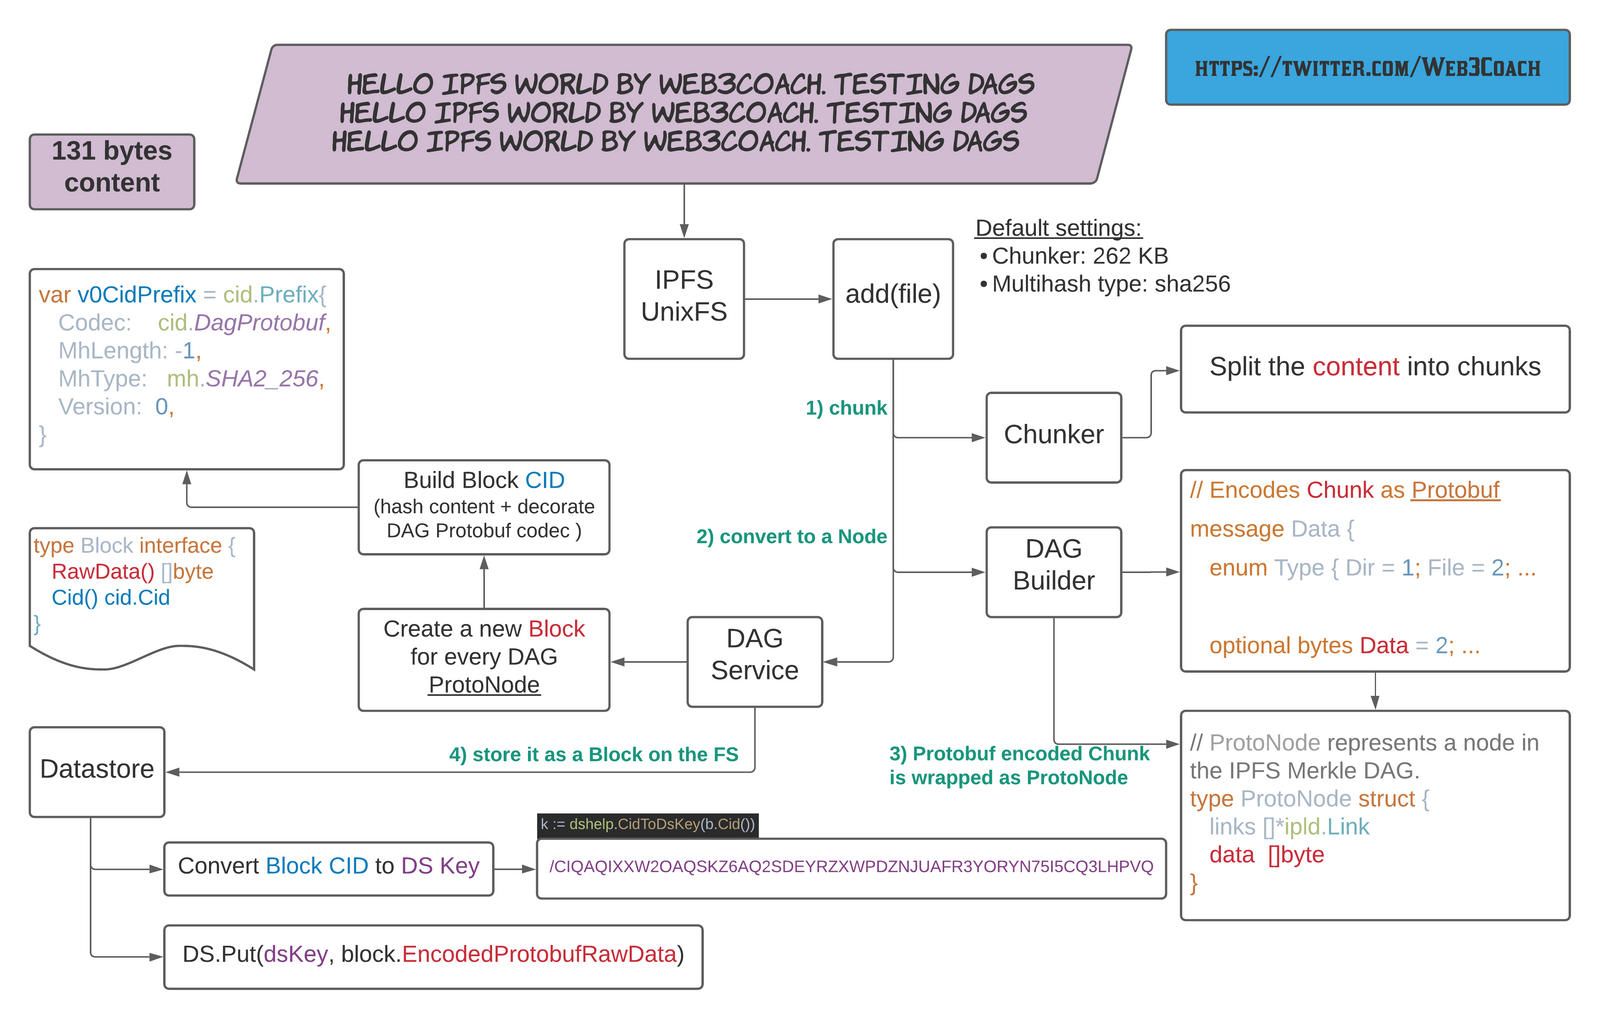
\includegraphics[width=\textwidth]{ipfs_algorithm.png}}
{IPFS algorithm.}


\subsection{Need for IPFS protocol}

Web 3.0 is a long-term target that aims to replace the current internet infrastructure. As decentralization is the essence of Web 3.0. Many consider the distributed ledger technology (DLT), for example, blockchains, as the core building block of Web 3.0. A blockchain is an immutable and append-only ledger that stores the network state. Distributed consensus between all the network nodes is required in order to extend the blockchain and store the critical network data among the network nodes. Therefore, it could be prohibitively expensive to store any other kinds of data into the blockchain. For multiple use cases, it may be more efficient to store other non-critical data in a secure fashion close to the security level of the blockchain. \\[-8pt]

IPFS is the most suitable storage medium for this category of data. IPFS allows for distributed storage of data that is immune to altering and forgery. Data stored on the IPFS network cannot be altered without changing the data identifier. In IPFS, the identifier is a cryptographic hash of the data. This means non-critical data can be stored to IPFS while storing this identifier to an underlying distributed ledger. This would result in less exhaustive operations over the distributed ledger. \\[-8pt]

\subsection{The Optimal Storage Platform for dApps}

Decentralized applications (dApps) are a class of applications that leverage decentralization to achieve unprecedented benefits. Among those are decentralized exchanges and marketplaces where centralized intermediaries are removed, hence eliminating/reducing any trading fees. Another example is decentralized social media and video platforms where content cannot be censored at the will of the operating company. Such dApps require the storage of a significant amount of data. IPFS allows this data to be stored in a distributed way that is censorship-resistant. For these reasons, IPFS is turning into a preferred storage platform for dApps.